\chapter{相关研究}
本章介绍本文相关研究工作,主要包括本体和问答的研究现状。首先介绍本体相关内容,包括本体核心构成要素:个体、类、属性、关系和本体描述语言;然后介绍本体构建方法研究和知识库问答的主流方法,包括基于语义解析的方法和基于信息检索的方法;最后介绍本文的工作与已有工作不同之处。

\section{本体构成要素}
从计算机科学角度看,本体是对相关领域知识的一种高度结构化、层次化的抽象建模,这种建模表示包含一系列计算机可以处理的形式化定义\cite{Hitzler}。运用本体可以很好地表示出领域中核心概念的语义信息和概念之间的相互关系。通过4个核心要素个体(Individuals)、类(Classes)、属性(Properties)及关系(Relationships),本体能够将领域知识以一种类似现实世界的组织方式形式化地表示出来,并且从某种程度上,既符合人的直观对领域知识层次分类的理解,又适合计算机存储、检索和推理。因此,本体是一种很好的结构化知识库建模方式。

\subsection{个体(individuals)}
个体,又叫实例(instances),是本体中最基本、最底层的组成单元。本体大多数描述都是企图更准确、更详细的描述出个体的信息特征。常见的人、动物、汽车、天体、星球等中的具体对象都可以看做个体,如地球、月球、太阳都是个体,就算是抽象的数字、单词等也可以视作个体。本体的一个很重要任务就是对本体领域中的个体进行层次化的分类,使得不同个体可以很好的进行区分或者是使其可以建立某种关系。

\subsection{类(classes)}
类,又叫类型(type)、类别(sort)、种类(kind)或者类目(category),常常指某个个体的上层延伸或者内涵。类是一些特征相似的个体构成的一个集合,或者是由一些子类构成的大类集合。如下为类的举例:

(1)人:人包括黄种人、白种人等类型,具体的张三、李四是人的个体。

(2)动物:动物包括无脊椎动物和脊椎动物两大类。

(3)汽车:汽车表示所有具体品牌汽车的类别。

(4)天体:天体包括地球、月球、彗星、流星等宇宙空间的物质。

(5)行星:行星包括地球、金星、木星、水星、火星、土星、天王星、海王星等。

通常情况下,一个个体可以属于不同的类别,这样使表达更灵活、表达力更强。同时,一个类可以包含其它类或者被其它类包含,这样构成了类的层次关系。一个类A被另一类B包含称为:A \textit{is subClassOf} B,通过这个关系可以得到很重要的性质,即B类具有的性质A类也同样具有。同样,一个类可以被多个类包含,也就是说一个类可以有多个父类。正是类别的上述层次关系,使知识不仅可以表示其自身的特征,还可以表示其与其它知识的关系,而且这种关系是非常接近人类的概念思维,所以知识建模很直观、易于理解。

\subsection{属性(Properties)}
属性用于表示个体间的关系(ObjectProperty)或者个体与其数据值之间的关系(DatatypeProperty)。例如人相关的属性\textit{hasWife}、\textit{hasHeight}和\textit{hasAge},\textit{hasWife}表示两个人(两个具体的人是两个个体)之间是夫妻关系,\textit{hasHeight}和\textit{hasAge}表示一个人的身高和年龄,身高、年龄值为数值类型。同样,属性与类结构类似,具有子属性层次结构。

属性的另外一个重要特点是:属性含有定义域(domain)、值域(range)的限制(restriction)。运用属性的这一限制,可以对属性两边的个体做相关的类别推理。如根据申明两个个体是\textit{hasWife}关系,可以推导出这两个个体的类别都是人,且更进一步该关系左边的个体类别为男人,右边的个体类别为女人。

\subsection{关系(Relationships)}
关系用来表示对象之间是以怎样的方式相联系在一起的。以汽车系列举例:“福特探险者是福特野马的下一代”,此例子体现出“福特探险者”和“福特野马”这两个对象存在着“下一代”的关系,这一事实可以表示为:

\begin{center}
	“福特探险者 \textit{is defined as a successor of} 福特野马”
\end{center}

此关系表达出“福特探险者系列”取代了“福特野马系列”这一事实,显然这种关系是存在着方向的。同样可以用此关系的反向关系,即“上一代”来表示上面的事实——“福特野马是福特探险者的上一代”。关系的总集合就构成了领域本体的丰富语义信息,因此关系的表达能力大小很大程度决定着本体对领域的抽象建模能力。如下介绍两种重要的关系:

(1)包含关系(subsumption relation)

包含关系主要有\textit{is-a-superclass-of}、\textit{is-a-subclass-of}和\textit{is-a-subtype-of},分别表示父类关系、子类关系和子类型关系。这些关系都是表达一种上下位的关系,特别是其中的\textit{is-a-subclass-of}关系,它体现出一种很强的分类学思想,可以直观地对领域概念进行分类,并且表示出这些类别的层次关系。

(2)总分学关系(mereology relation)

总分学关系指的是一种部分(\textit{part-of})与整体的关系,表示一个对象是另一个复合对象的一部分。还是以“福特探险者”系列为例,“方向盘 \textit{is-a-part-of} 福特探险者”,表示方向盘是福特探险者汽车的一个部件。

除了包含关系和总分学关系以外,本体中还有一些其它的关系,这些关系不一定表示层次关系,其往往是该本体领域中的特定业务关系。这种领域的特定关系被用来表达领域独特的事实知识,构成了自身领域本体的特色,因此不同领域本体表示往往差别比较明显。

\section{本体描述语言}
使用本体描述语言可以很好的对领域本体进行层次化的表示。常见的本体描述语言有:Ontolingua、OCML、OKBC、FLogic、LOOM、DAML、SHOE, OIL、XOL、XML、RDF、RDFS、OWL\cite{Corcho}。其中,由W3C推荐的XML、RDF、RDFS以及OWL使用最为广泛。

XML(Extensible Markup Language)\cite{xml}是一种标记语言,通过其标记可以对结构化文档进行分层的语法表示,并且易于机器处理和人类阅读。然而,XML标记缺乏对文档的含义进行约束,标记内部也缺乏结构化定义,因此很难充分描述出本体中的四个常见核心要素。RDF(Resource Description Framework)\cite{rdf}是一种描述对象(资源)以及对象之间关系的图数据模型,其兼容XML语法,并且含有简单的语义。RDFS(RDF Schema)\cite{rdfs}是扩展的RDF词汇表,这里的词汇表指定义为个体、类、属性和关系的术语名称。RDFS通过扩展了RDF中没有的属性和类层次结构语义,也即通过定义子属性(subPropertyOf)、子类(subClassOf)、属性定义域约束、属性值域约束来增强描述资源的表达能力。尽管RDFS相对RDF的描述资源能力更强,RDFS仍然是一种相对简单的本体语言,其描述资源能力依然很有限\cite{gao}。例如:RDFS无法描述类的不相交关系,如类“男人”和“女人”是不相交的,但其只能描述“男人”和“女人”同属于“人”;同时,RDFS也无法描述类的布尔组合(并集、交集、补集)关系,如“人”无法定义成“男人”和“女人”的并集等。为弥补RDFS表达能力的不足,W3C又推出了表达能力更强且具备强推理能力的本体语言——OWL(Web Ontology Language)\cite{owl},OWL定义了逻辑类的关系表示,即提供了针对逻辑与、或、非的领域关系表示,可以有效的表示类的并集、交集、补集运算,因而可以表达更复杂的本体知识。

OWL的一个很重要设计思想是在知识表达能力和推理效率之间找到一个平衡。因此,在其不同的表达能力和推理效率设计中,为满足不同用户对本体建模需求,又诞生了三个子语言,即OWL Lite、OWL DL(Description Logic)和OWL Full。这三个子语言描述能力依次增强,推理复杂度逐渐提高。OWL Lite更关注本体表达的简洁性,其表达能力相对其它两种语言较弱,但其推理最高效,因此OWL Lite更适合于对表达能力要求不是太强的领域;OWL DL比OWL Lite表达能力更强,与OWL Full比具有计算完备性(所有结论均可计算)和可判定性(有限时间内所有计算均可终止),同时OWL DL支持有效的推理,因此在既对本体语言表达能力要求高,又保证推理可判定性时,可以选择此语言;OWL Full的表达能力最强,正因其表达更灵活、约束较少,也使其推理不可判定,但OWL Full有完全兼容RDF的优点,这也是前两种语言不具备的,因此在以兼容RDF为主要建模目标的场景,OWL Full语言是较好的选择。

\section{本体构建方法研究}
目前,本体构建方法\cite{yue}主要有两种:第一种是在领域专家的指导下,使用本体描述语言表示领域本体;第二种是从结构化、半结构或者无结构数据抽取本体要素,形成领域本体。第一种本体构建方法往往采用纯人工方法,由于人的主观性,不同领域专家构建出来的本体常常相差很大且构建效率低。但从局部来看,专家构建的本体知识质量很高,专家站在领域高度对知识进行了专业化的总结、提炼,知识表达更准确、合理。所以,在对知识表示专业程度要求很高、知识数量较小的领域(如高考地理解题),此方法可以达到很好的效果。第二种本体构建方法是为了缓解第一种方法中的人为主观性和低效性而提出的,其使用自动或者半自动的方法构建本体,既节省时间又提高了知识表示的一致性。该方法很大程度依赖于自动、半自动技术的能力,构建出来的本体往往噪音较多、抽象程度不高(知识没有经过深度提炼、总结)。因此,在一些对知识准确度要求很高的场景,如地理高考解题本体构建等,此方法不是很适合,但是在一些对噪音容忍度比较高的场景,如通用领域的本体构建,此方法运用很广且效率很高。

由于本文构建用于辅助解答高考地理多选题的本体,其知识要求精炼、准确、少噪音且知识量不大(只包含核心地理高考考点),因此需要地理领域相关专业人士人员构建,保证质量。本文也只详述人工本体构建的研究现状,对于自动和半自动本体构建方式的研究现状,本文不加以叙述。

国内外常见人工本体构建方法有:IDEF5法\cite{IDEF5}、骨架法\cite{skelton}、TOVE法\cite{TOVE}、METHONTOLOGY法\cite{METHONTOLOGY}、KACTUSK工程法\cite{KACTUSK,KACTUSK2}、SENSUS法\cite{SENSUS}以及七步法\cite{seven}等。IDEF5法、骨架法及TOVE法常用于企业领域本体构建。IDEF5法使用图表以及很细化的说明形式来获取企业业务存在的概念、属性及关系,从而形成本体;骨架法是一种流程图导向的本体构建方法,其描述的是一种本体构建的方法框架;TOVE法是通过本体建立企业知识的逻辑(一阶逻辑)模型。其它四种方法用于构建领域知识本体。METHONTOLOGY法是在构建化学元素周期表本体基础上发展而形成的通用本体构建方法,此方法偏向软件工程的思想,本体的构建也引入了管理、开发和维护三个很具软件工程特征的阶段;KACTUS法是对应用驱动的本体开发方法,侧重对已有本体的复用和扩充方法;SENSUS法提供一种自顶向下的层级结构本体构建方法,偏向操作性指导。七步法是基于本体工具protege\footnote{https://protege.stanford.edu/}的构建方法,主要分七个步骤构建本体,比较偏向实用性、操作性。具体七种本体构建方法比较如表2.1所示。

\begin{center}
	\begin{small}
	表2.1:七种本体构建方法比较
	\end{small}
\end{center}

\begin{figure}[!htb]
	\centering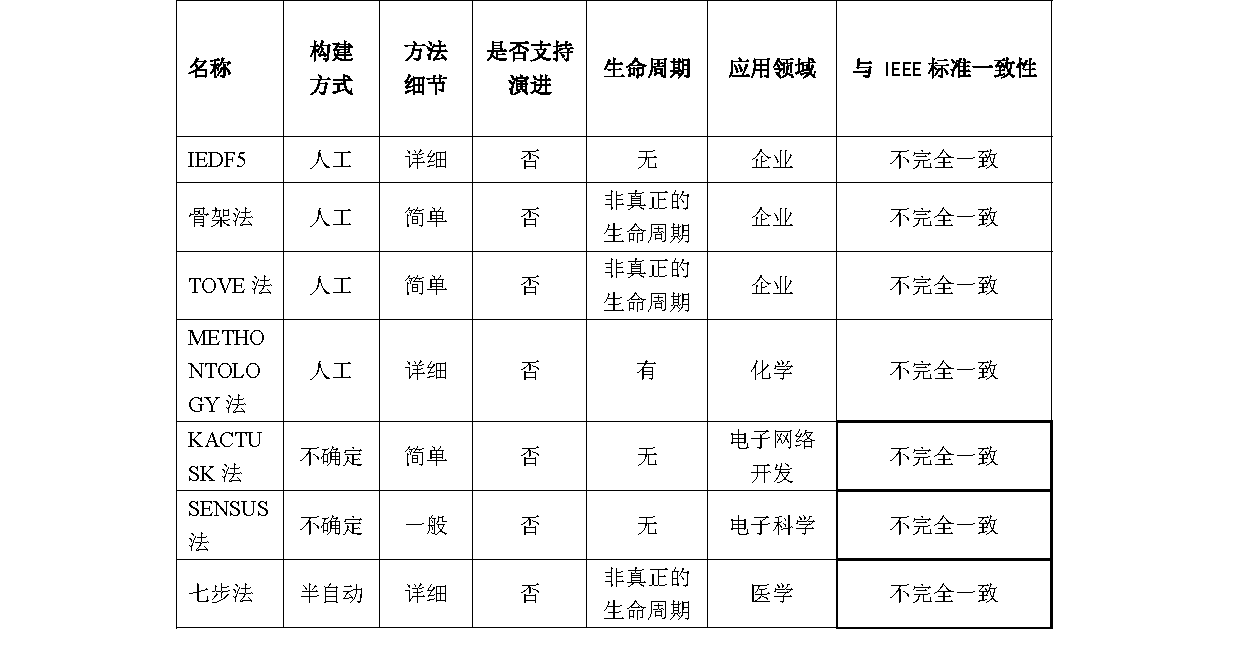
\includegraphics[height=7cm]{resource/onto_method_compare}
	\label{fig:onto_method_compare}
\end{figure}

分析以上七种人工本体构建方法可知,这些构建方法都缺乏对本体进化的考虑,本体只立足当下情况,没有考虑后期本体的更新,也使本体知识不能与时俱进。同时,这些方法人工参与力度很大,使用的技术较简单,构建时并没有统一的标准规范对其指导,构建人员均需从自身领域特点出发进行扩展与缩减。因此,本体构建方法相差还是比较大,这也表明统一的本体构建规范、评价标准还不成熟。

\section{问答方法研究}
问答是人工智能领域中的一个热门的研究问题,它综合运用了各种自然语言处理技术。对于用户提出的某一个问题,问答系统往往可以给出简短、精准的答案组织形式,而非一系列的相关网页文档供用户参考,省去了用户额外从大量的相关网页文档中寻找所需确切信息的时间\cite{Lu} \cite{Bertola}。同时,问答技术集成了定位、抽取以及表示出针对用户提出的自然语言问题答案的丰富功能,因此受到广泛的关注\cite{Abacha}\cite{Pavli}。

问答一般分为两类:开放域的问答和封闭域的问答。开放域的问答又叫无结构数据的问答,一般是从开放的网页或者文档中抽取所需的问题信息。封闭域的问答又叫受限域的问答或结构化数据的问答,其往往需要预先定义的知识源,例如领域本体或关系数据库管理系统\cite{Dalmas}\cite{Dragoni}。 查询数据库的方式有两种,第一种为结构化查询,如SQL,另一种为自然语言查询,即用户用自然语言组织其问题,而不需要一些专业术语的限制\cite{Jagadish}。结构化查询虽其功能强大,但不易使用,对缺乏训练的普通用户不友好。相反,自然语言查询方式对用户更友好,用户可以轻松组织自然语言进行复杂的问题查询。

对于知识问答而言,其强调如何根据给定问题作出精准回复,其答案要求不能包含无效的信息。因此,知识问答的知识源常常选取高度结构化、包含丰富语义信息的数据,如本体等。建立于高度结构化数据之上的问答也叫做知识库问题,本文将详述知识库问答的主流研究方向和方法。

目前,知识库问答(knowledge base question answering,KBQA)主要有两个主流的研究方法:基于语义解析、基于信息检索。分别如下介绍:

\subsection{基于语义解析的KBQA}
基于语义解析的方法一般先构建一个语义解析器,然后运用该语义解析器将自然语言问句转换为特定类型的逻辑表达式,如带类型的 lambda 表达式(typed lambda calculus)、 lambda依存组合语义。以问题“姚明的老婆出生在哪里?”为例,问题经过构建的语义解析器解析过后,可以表示为如下lambda 表达式:
\begin{center}
$\lambda x.$配偶(姚明, y)\space$\wedge$ 出生地(y, x)
\end{center}

在此lambda表达式中,$\lambda$.x表示该表达式的变量x,关系配偶(姚明, y)表示姚明的配偶(也即问题中的老婆)y,关系出生地(y, x)表示y的出生地是x,$\wedge$表示上述两个关系同时满足,整个句子表达的含义也就是“姚明的配偶的出生地”,即为题中问题“姚明的老婆出生在哪里?”的一种较正式表达。

传统的语义解析器需要有人工标注的逻辑表达形式作为监督知识,并且它们是在特定领域(受限域)进行相关操作,逻辑谓词的数量也较少\cite{Zettlemoyer}\cite{Wong}\cite{Kwiatkowski}。Zettlemoyer和Collins在研究将美国地理领域问题(Geo880\footnote{http://www.cs.utexas.edu/users/ml/geo.html}中问题)表示成lambda表达式时,使用人工标注的问题和对应逻辑表达式作为训练数据,去学习语义解析器,而且研究中定义的领域谓词也很有限,如类型、大小、多少、边境、城市、州、河流等。

由于获取人工标注的逻辑表达式进行有监督的训练语义解析器代价太大,并且人工标注的量始终有限,因此有相关研究尝试在不需要人工标注的逻辑表达式的前提下,学习一个语义解析器。Berant\cite{BerantCF}等人训练了一个适应freebase的语义解析器,该研究主要分两步进行:第一步是构建较完备的词汇表,第二步是桥接(Bridging)操作。构建词汇表也就是将自然语言与知识库实体或实体关系进行单点映射,也可称作对齐(alignment),自然语言实体到知识库实体的匹配较简单,可以使用一些简单的字符串匹配方式,如“Obama was also born in Honolulu.”中Obama映射到Barack Obama,但是要将例句中的自然语言短语“was also born in”映射到相应的知识库实体关系PlaceOfBirth, 则较难通过字符串匹配的方式建立映射。此处作者使用一种远程监督的思想,作者使用开放信息抽取软件ReVerbopen IE system\footnote{http://reverb.cs.washington.edu/}从ClueWeb12\footnote{http://lemurproject.org/clueweb12/}数据集上抽取15,000,000个三元组构成一个数据集,然后将短语对齐到知识库关系。完成词汇表的构建后,仍然有些轻动词(light verb),如go,where,do难以映射到知识库,比如“Which college did Obama go to?” 中的“go to”无法映射到知识库关系,因此作者使用“桥接”操作,从知识库中找出一个中间二元关系(本例中为Education)来将当前实体和关系连接起来。该研究在free917\footnote{https://github.com/pks/rebol/tree/master/data/free917}上取得了较好效果。

使用有监督的数据训练语义解析器在知识库数量较小时质量很高,但是很难适应大型知识库,如freebase等。Cai\cite{Cai}等人将直接根据标注的数据训练语义解析器的过程简化为三个子过程,以减小在遇到未见过测试数据时的失败率。这三个子过程分别是标准的监督学习算法、模式匹配(schema matching)和模式学习(pattern learning)。该研究应用现有的监督训练算法对有标签数据集进行语义解析,使用结构匹配技术查询自然语言词汇与本体知识库中符号的相关联性,使用模式学习技术将新的(自然语言词,本体词汇)对合并到训练的语义解析器中。此研究优点是将一个问题分解为了三个子问题,使之可以运用每个子问题领域的成熟技术。同时,三个子过程联合确定问题的逻辑表达式,比单纯的使用有监督的问题到逻辑表达式对训练,而得到的语义解析器可靠性更强。该研究在free917数据集比单纯的有监督学习语义解析器的算法F值高出0.42\%。

之前的研究在生成语义解析器时都很少运用到知识库的相关结构图信息,因此,问题中的词表达方式和知识库中术语的表达方式仍然相差很大,相互映射也比较困难。为了解决上述问题,并且充分利用知识库的结构信息,Yih\cite{Yih}等人提出了一个紧密结合知识库的语义解析器。作者定义了一个类似知识库子图的查询图(query graph),该图可以直接映射到一种$\lambda$演算,因此作者把问句的语义解析过程转化为查询图生成过程,并且转化为按阶段状态(stage state)和动作(action)的搜索问题,其中每个阶段状态是查询图表示中的候选解析,每个操作都定义了一种扩展关系图的方法。作者将动作分为三步,第一是识别问题中的主题实体,第二是寻找答案与主题实体之间的主要关系,第三是使用附加的、描述答案需要有的属性约束,或者是答案与问题中其它实体的关系来扩展查询关系图。这种方式通过将问句表达部分靠近知识库中的某些实体和关系,使得只需要关注最可能成为正确查询图的区域,使搜索空间大大缩小,搜索效率也大大提高。该研究在WebQuestions\footnote{https://nlp.stanford.edu/software/sempre/}上也超过了之前的方法,并取得较高的F值52.5\%。

\subsection{基于信息检索的KBQA}
基于信息检索的方法一般根据问题中的关键信息去知识库查询一批候选答案,然后运用排序打分技术对候选答案进行打分,选出得分最高的候选答案。具体的操作如下:

(1)识别问题中的主题实体,即问题考察的核心实体。

(2)根据问题主题实体,从知识库中查询该实体以及其相关联的实体子图,子图的边作为候选答案集合。

(3)使用规则或者模板等,人工或者自动、半自动地构建问题的特征向量,然后根据问题特征向量对候选答案进行筛选。或者直接对问题和候选答案进行分布式的表示,即对问题、答案进行向量建模,然后根据问题、答案的向量相似性来筛选最终答案。

Yao和Van\cite{Yao}首先将信息检索方法运用到知识库freebase\footnote{https://developer.google.com/freebase}问答上,其使用了信息抽取的技术。该研究首先使用Standford CoreNLP\footnote{http://nlp.stanford.edu/}构造出问题的语法依存树(dependency tree),然后识别问题中的问题词(如what、who、when等)、问题焦点词(常暗示着答案的类型词,如name、place等)以及通过命名实体识别来确定主题词,通过词性标注获取问题的中心动词。再然后,根据主题词找出知识库中对应的主题词的子图,包含跟主题词相关联的实体结点边,所有实体结点的边构成问题候选答案三元组集合。最后,选取候选答案实体结点的关系、结点属性构成候选答案的特征向量,并使用问题和答案特征向量构建一个逻辑回归分类器。总体说来,此方法也运用到一些语言学知识,但总体还是较符合人的直觉。

为解决问题、答案抽取特征向量时对语言学知识和人工规则的依赖,一些研究尝试使用语义向量来对问题、答案进行分布式表示(Distributed Embedding)。Bordes\cite{Bordes3}等人率先使用基于神经网络的方法在开源知识库 ReVerb\cite{Fader}上进行问答任务。Bordes等人将问题和知识库三元组都表示成低维向量,并且使用余弦相似度来计算出与问题最相近的答案。问题和答案的表示使用词袋法(Bag Of Words,BOW),使用成对的训练(pairwise training)方法,即一个正例随机选取多个知识库中的事实反例进行训练。Bordes\cite{Bordes1}等人意识到仅仅使用自身的答案三元组表示答案向量过于简单,因此引入答案结点的子图,选取与结点距离一跳1-hop\footnote{直接与结点相连的结点,即与结点路径长度为1的结点}和两跳2-hop\footnote{与结点路径长度为2的结点}的结点,将子图结点的关系以及结点本身信息都加入到答案结点,从而更综合的表示答案结点,此处向量的表示仍采用BOW方法,该结合子图表示的方法也一定程度上提升了问答性能。

注意到Bordes等人BOW方法表示问题、答案的缺陷,BOW方法忽略问题中信息的先后顺序,对于复杂问题表达能力不够,并且Bordes等人的模型没有考虑对问句类型进行分析。Dong\cite{Dong}等人试图通过从问题的不同方面来表示问题、答案向量,他们考虑从三个方面理解问题,即问题的答案路径(answer path)、问题的答案上下文(answer context)和问题的答案类型(answer type)。问题的答案路径指答案结点和问题主题实体之间的关系集合;问题的答案上下文指与答案路径直接相连的实体集合和关系集合;问题的答案类型指答案的数据类型或者结点类别,如答案为时间类型或类别人等。Dong等人使用三个不同参数的CNNs(Convolutional Neural Networks)分别表示问题的这三个方面向量,同时也表示答案的这三个方面向量,最后用问题和答案这三个方面对应向量的内积操作和表示问题和答案的相似度,用来选择最为相似的候选答案。

上述方法都是在试图根据问题或者答案的相关方面来更加综合的表示问题或者答案。从实质上来说,问题的表示和答案的表示都是单独进行,也就是说问题的表示没有参照当前的候选答案信息,候选答案的表示也没有参照当前的问题信息。

随着深度学习技术的进一步发展,在神经机器翻译领域(neural machine translation, NMT),一种注意力(Attention)机制被证明在机器翻译任务上面有不错的性能提升。如Bahdanau\cite{Bahdanau}等人将Attention运用到传统的基于编码-解码(encoder-decoder)簇的机器翻译中,传统的解码器在生成翻译词的时候是将源句子表示成固定长度向量,该研究猜想将源句子表示成固定长度可能是性能提升的瓶颈,因此提出了注意力机制,在预测翻译目标词的时候,通过注意力模型自动地搜索与目标词相关的源句子中的部分词。在英语到法语的翻译任务中,该研究取得了较好的性能。

Luong\cite{Luong}等人更进一步研究了两种类别的注意力机制(全局注意力、局部注意力)在机器翻译任务上的效果。该研究使用全局注意力每次都关注整个源句子词,使用局部注意力每次只关注源句子中的部分词,该研究也证实了这两种注意力机制对英语到德语的翻译均有效,最终该研究使用两种注意力的集成模型,在WMT'15\footnote{http://www.statmt.org/wmt15/translation-task.html}英语到德语的翻译任务上,取得了较好的性能效果。

除了机器翻译任务,注意力机制也被运用到句子级别的摘要(sentence-level summarization)任务上,并取得了一定的性能提升。Rush\cite{Rush}等人将局部注意力机制运用到句子摘要任务中,在生成每个摘要词的时候对齐源句子中的部分关键词,在DUC-2004\footnote{https://duc.nist.gov/duc2004/tasks.html}任务上,也取得了高于baseline的性能提升。

受到注意力机制的启发,有研究将注意力机制运用到知识库问答中,通过注意力机制动态的根据答案向量表示问题向量或者根据问题向量表示答案向量,避免了之前工作中独立表示问题向量和答案向量的缺陷。liu\cite{Liu}等人根据问题每个词对答案的注意力分配来综合表示问题。该研究首先将答案向量表示成四部分,即答案实体(answer entity)、答案关系(answer relation)、答案类型(answer type)和答案上下文(answer context,该论文中为与答案实体直接相连的实体集合),然后问题中每个词的表示根据答案四个方面的综合注意力权重求和,最后使用问题相对答案四个方面的表示向量与答案的四个方面向量求内积和得到问题、答案的相似度,并根据设定的答案相似度边距(margin)来确定最终答案。该文献中为解决未登陆词(out of vocabulary, OOV)问题,加入全局的知识库作为训练的知识源。该研究在freebase知识库问题任务中取得了同类基于信息检索的方法中较好的性能。Tan\cite{Tan}等人将注意力机制运用到深度学习模型中回答非事实型问题。该研究先是通过基本框架双向循环神经网络模型来表示问题、答案的分布式词向量,然后在答案的表示时,使用注意力机制来根据问题的内容生成答案向量,最后根据问题、答案的余弦值计算两者的相似度。在TREC-QA\footnote{https://trec.nist.gov/data/qa.html}和InsuranceQA\footnote{https://github.com/shuzi/insuranceQA}任务上,此研究模型的实验效果超过了一些baseline模型。

通过以上对基于语义解析的KBQA和基于信息检索的KBQA的方法分析可知,虽然基于语义解析的方法具有一定的有效性,但它们很大程度上受限于外部资源的质量,而且需要大量的特征工程工作,再者引入大量语言学知识会大大增加系统复杂度。而基于信息检索的方法更简单,不需要使用大量的人工特征和语言学特征,实现也更灵活,在开放域知识库Freebase上的问答研究实验也表明,该方法可以达到与基于语义解析方法相近的F值\cite{Dong,Bordes2},因此基于信息检索的KBQA运用比较广泛。

\section{本文与已有工作不同}
本文两个主要任务为构建地理本体CGeoOnt、根据构建的地理知识库构建问答系统,本节分别从这两个任务阐述本文与已有工作的不同。

对于构建地理本体CGeoOnt任务,本文参照高考地理考题的考察方式组织,一些术语的名字组织也并不是仅仅根据地理教材中的名称,更不是凭主观想象,而是从更方便解题角度组织。再者,地理本体CGeoOnt中含有很多特殊元素,如静态属性,专门为类添加的属性描述,类的静态属性性质默认施加到类的实例上。还有地理中的过程表示,地理中的大量现象形成很复杂,很多是带有条件、过程性的,本文针对地理过程也定义了一下特殊的词汇描述,这也是一般的本体构建中没有的。正是因为地理知识组织的复杂性,本文的一些本体元素组织往往超过了一般本体语言的语法定义,本文也针对做了扩充(如添加静态属性),因此本文也不太适合用一般的本体构建工具,如protege等,本文需要开发自己独特的本体解析工具。

对于基于地理知识库的问答任务,从本文收集的web地理问题分析可知,地理问题表达形式多样,一个地理三元组知识往往可以成为多个问题的答案,如“亚热带季风气候在发展农业生产方面有什么优势” 和“温带季风气候在农业生产方面的显著优势是\_百度知道”,这两个问题都可以用“季风气候$\space$生产优势$\space$夏季高温多雨,雨热同期。”这个三元组知识作为答案。虽然,两个问题问法不同,但相对答案而言它们等效。这也说明,在我们做问答时,单独的表示问题和答案向量是不充分的,至少是不能表示问题和答案之间的关系。因此,本文在表示地理问题、答案时,充分考虑到了两者的内在关联。再者,本文地理问题本身表达方式偏口语化严重,其更具挑战,且问题中无关信息很多,对答案和问题的表示要求更高。

最后,目前中文地理问答数据集缺乏,为了验证实验的有效性,本文还需构建客观、真实、多样化的web地理问题、答案对数据集。

\section{本章小结}
本章介绍了基于本体的地理知识问答的相关研究现状。具体包括本体构建的研究现状和知识库问答的研究现状。本章首先介绍本体的四个基本元素个体、类、属性、关系和常见的本体描述语言;然后介绍本体构建的主流方法,主要是介绍八种常见的人工本体构建方法的优缺点和适合范围;再然后介绍知识库问答的两个主流方法——基于语义解析的KBQA问答和基于信息检索的KBQA的操作流程以及各方向的研究方法优缺点;最后介绍本文工作与已有工作的不同之处。
